% Sample of a report for an attack as requested at wednesday, 5 December 2018, mail "Assignemnt Lab 19"
\subsection{Ping of Death}
% Introduction about this attack
\subsection{Introduction}
An IP packet has a maxiumum length of \textit{65535 bytes} $(2^{16}-1)$ as described in the relative \href{https://tools.ietf.org/html/rfc791}{RFC 791}.\\
So it's not possible to send an IP packet that has a length more larger than that length, but it is possible to send the packet fragmented in plus that one.\\
The receiver could be crash reassembling the packet.\par

% SCAPY program
\subsubsection{SCAPY program}
\lstinputlisting{scapy/PingOfDeath.py}

% Wireshark presenting  the attacker's messages
\subsubsection{Attacker's messages}
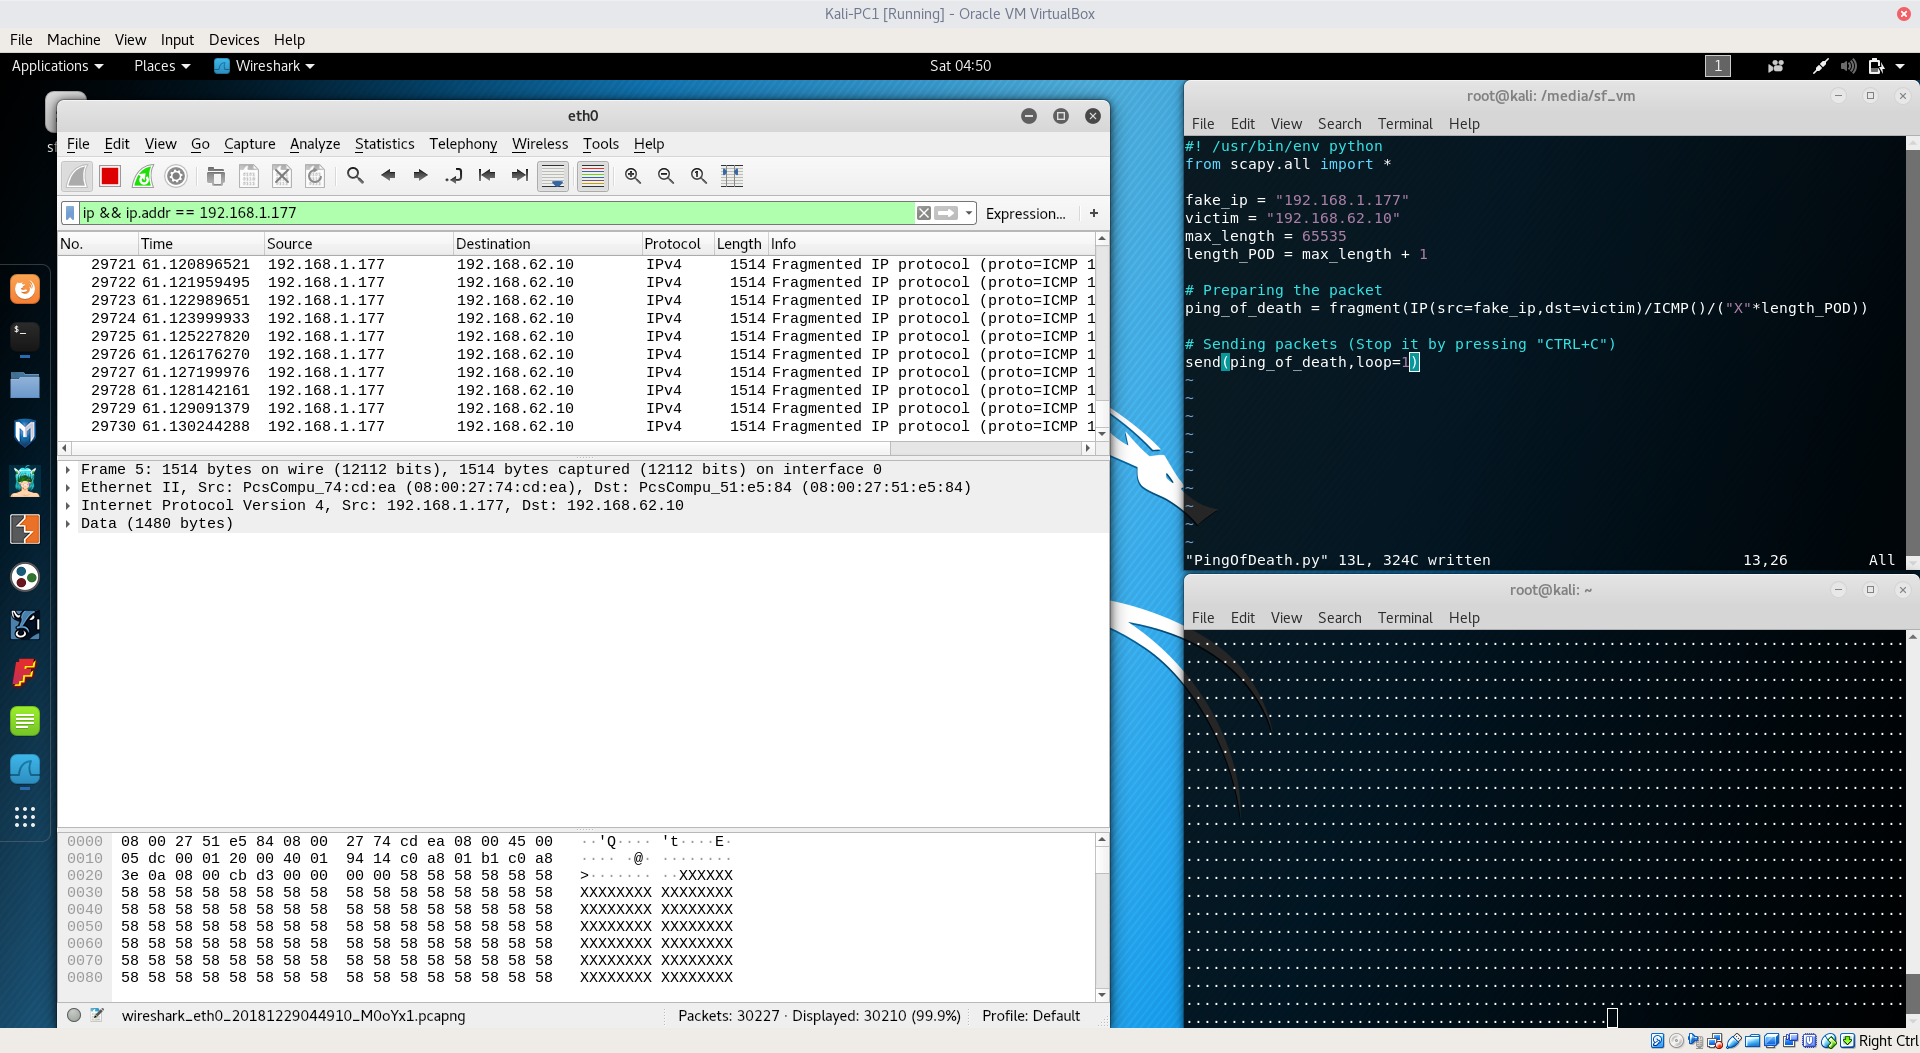
\includegraphics[width=16cm]{img/PingOfDeath.png}

% Explanation of the result of the attack
\subsubsection{Attack's result}


% Method recommended to protect the Network against such an attack
\subsubsection{How to protect the network}
In order to avoid this attack it could be useful check all incoming IP fragment to recognize if the sum of the "fragment offset" and the "total length" of the IP packet is regular. If not the packet it could be considered invalid and so it could be rejected.\par
